\chapter{Conclusão} 

\section{Discussão dos Resultados} 

As classes destinadas à implementação da interface no framework android fornecem
acceso a recursos que servem para implementação de responsabilidades não
relacionadas com a interface. Essa característica do framework android leva à
implementação da camada de View com diversas responsabilidades que não são
inerentes à interação com o usuário. Isso dificultou a refatoração, pois as
classes que exercem o papel de Presenter necessitam interagir com as classes de
View para acessar esses recursos, além de atualizar o estado da View. O uso do
padrão de injeção de
dependência\footnote{Padrão
de projeto onde um objeto recebe as referências para as suas dependências sem
conhecer os processo de contrução das mesmas.
\url{http://en.wikipedia.org/wiki/Dependency_injection}}
pode ser aplicado para acessar esses recursos e serviços sem a necessidade de
interação com a classe de View. A figura \ref{fig:classes_iteracao3} mostra a
disposição das classes após a refatoração.


\begin{figure}[!h]
	\centering
	\label{fig:classes_iteracao3}
	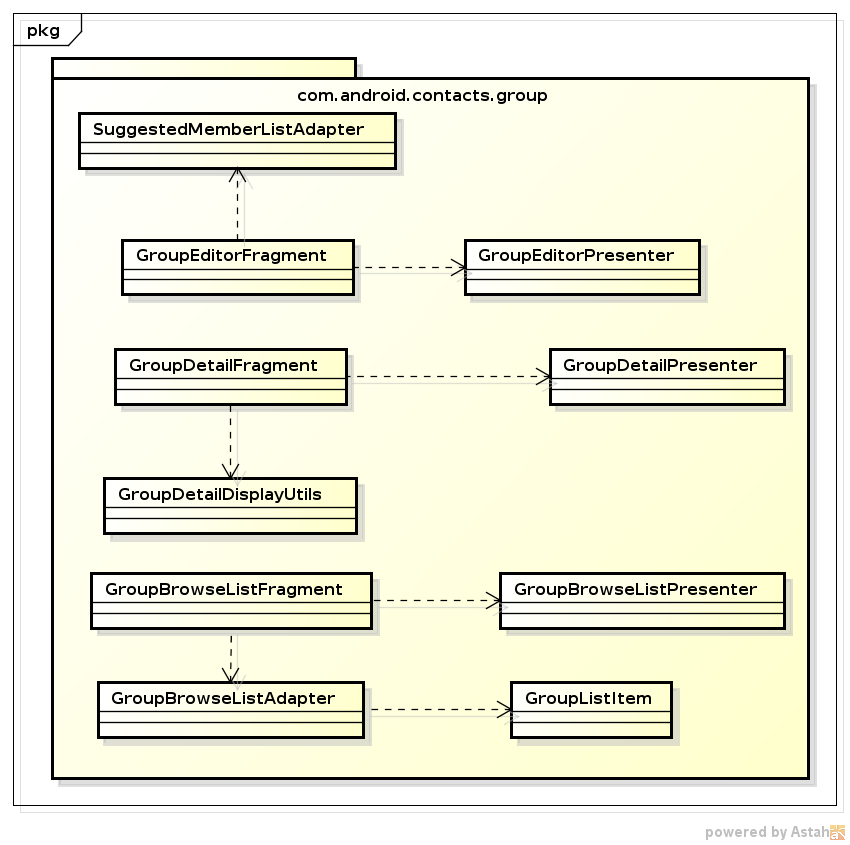
\includegraphics[scale=0.55]{img/classes_iteracao3}
	\caption{Pacote após refatoração/Fonte: Próprio autor}
\end{figure}


Ao usar o padrão MVP, a granularidade dos métodos aumentou pois cada um dos
componentes implementaram uma parte do caso de uso aumentando o números de
métodos que se reflete na métrica WMC, isso afeta também a métrica RFC pois
esses métodos estão relacionados entre si, aumentando a troca de mensagens entre
a View e o Presenter. Um ponto positivo sobre isso é o fato de que métodos 
complexos com muitas linhas de código foram desmembrados em métodos menores e
mais simples, implementados tanto na View como no Presenter.

Houve diminuição na métrica CBO nas classes alteradas pois diversas
responsabilidades que utilizam essas dependências foram movidas para a classe de
Presenter. Analisando de forma geral, essas dependências permanecem no pacote
além de ser criado mais um acoplamento entre a View e a nova classe Presenter.

A métrica WMC está relacionada com as métricas DIT e NOC. Como houve pouca
variação no DIT e nenhuma variação no NOC o aumento da WMC não tem impacto
relevante. Entretanto a métrica RFC aumentou indicando maior complexidade. Os
resultaddos mostram que isso se deve à melhora da coesão do código demonstrado pela
diminiução da métrica LCOM. Comforme um software é desenvolvido novas classes e
troca de menssagens são implementadas afetando as métricas WMC e RFC. 

Não existe valores ideais para as métricas e seu maior valor está em identificar
anomalias que devem ser analisadas caso a caso. Como não houve uma refatoração
mais extensiva do projeto não é possível determinar valores de referência para
as métricas. 

Não é possível relacionar diretamente a métrica CBO com base na
variação dos resultados para esta métrica, apesar de que, os valores se
mantiveram abaixo dos encontrados da versão de referência.
Isso requer mais estudos abordando outros padrões de projeto. 

Os experimentos demonstraram que a aplicação do padrão MVP promoveu de forma
significativa maior coesão no aplicativo. Isso é demonstrado nos resultados da
métrica LCOM que foi a mais afetada pelo uso do padrão MVP no projeto como pode
ser observado na figura \ref{fig:allmetrics}.

\begin{figure}[!h]
	\centering
	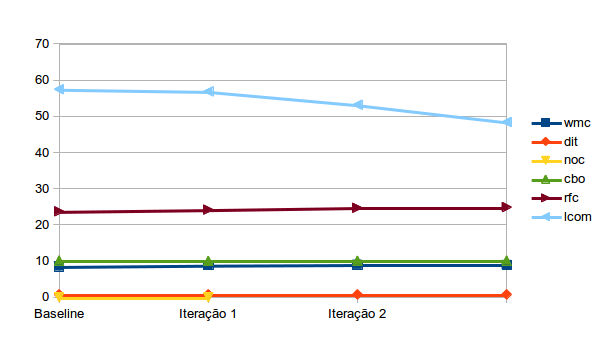
\includegraphics{img/allmetrics}
	\caption{Variação das métricas ao longo das iterações/Fonte: Próprio autor}
	\label{fig:allmetrics}
\end{figure}

É possível obeservar nos resutados a relação entre LCOM e as métricas 
WMC,RFC que aumentaram conforme o LCOM diminuia. O aumento da complexidade
indicado pelas métricas WMC e RFC é pequeno em comparação à diminuição de
complexidade indicada pela métrica LCOM, pode se chegar a essa conclusão não só
analisando os resultados, como também ao analisar o código em que as classes
estão menores, mais coesas com responsabilidades bem definidas.Portanto, a
arquitetura proposta melhorou a qualidade do objeto de estudo porque promoveu
maior coesão e diminuindo a complexidade.

 
\section{Trabalhos Futuros}

Existem outros padrões de projetos para o desenvolvimento da camada de
apresentação de um software que não foram analisados nesse trabalho, a saber: 
MVVM, MVP-VM, MVPC. Essas variações no padrão MVC surgiram em contextos
diversificados e podem agregar algum benefício à qualidade do aplicativo.
Este trabalho não aborda o impacto do padrão MVP em outras métricas de qualidade
de código.
Não foi feita uma avaliação dos impactos na performance do aplicativo devido ao
uso do padrão MVP. A inclusão de mais objetos interagindo trocando mensagens
pode depreciar a performance, levando-se em consideração sua execução em
ambientes mais restritos, como no caso de um aparelho móvel.